% Digital Logic Report Template
% Created: 2020-01-10, Maya Martin

%==========================================================
%=========== Document Setup  ==============================

% Formatting defined by class file
\documentclass[11pt]{article}

% ---- Document formatting ----
\usepackage[margin=1in]{geometry}	% Narrower margins
\usepackage{booktabs}				% Nice formatting of tables
\usepackage{graphicx}				% Ability to include graphics

%\setlength\parindent{0pt}	% Do not indent first line of paragraphs 
\usepackage[parfill]{parskip}		% Line space b/w paragraphs
%	parfill option prevents last line of pgrph from being fully justified

% Parskip package adds too much space around titles, fix with this
\RequirePackage{titlesec}
\titlespacing\section{0pt}{8pt plus 4pt minus 2pt}{3pt plus 2pt minus 2pt}
\titlespacing\subsection{0pt}{4pt plus 4pt minus 2pt}{-2pt plus 2pt minus 2pt}
\titlespacing\subsubsection{0pt}{2pt plus 4pt minus 2pt}{-6pt plus 2pt minus 2pt}

% ---- Hyperlinks ----
\usepackage[colorlinks=true,urlcolor=blue]{hyperref}	% For URL's. Automatically links internal references.

% ---- Code listings ----
\usepackage{listings} 					% Nice code layout and inclusion
\usepackage[usenames,dvipsnames]{xcolor}	% Colors (needs to be defined before using colors)

% Define custom colors for listings
\definecolor{listinggray}{gray}{0.98}		% Listings background color
\definecolor{rulegray}{gray}{0.7}			% Listings rule/frame color

% Style for Verilog
\lstdefinestyle{Verilog}{
	language=Verilog,					% Verilog
	backgroundcolor=\color{listinggray},	% light gray background
	rulecolor=\color{blue}, 			% blue frame lines
	frame=tb,							% lines above & below
	linewidth=\columnwidth, 			% set line width
	basicstyle=\small\ttfamily,	% basic font style that is used for the code	
	breaklines=true, 					% allow breaking across columns/pages
	tabsize=3,							% set tab size
	commentstyle=\color{gray},	% comments in italic 
	stringstyle=\upshape,				% strings are printed in normal font
	showspaces=false,					% don't underscore spaces
}

% How to use: \Verilog[listing_options]{file}
\newcommand{\Verilog}[2][]{%
	\lstinputlisting[style=Verilog,#1]{#2}
}




%======================================================
%=========== Body  ====================================
\begin{document}

\title{ELC 2137 LaTeX Tutorial }
\author{Maya Martin}
\maketitle

\section*{Summary}

Students were required to insert and center a floating table with necessary numbers, manipluate a screenshot to fit properly, and list questions. By coding all of the following in Latex students are able to produce a professional report.


\section*{Q\&A}
\begin{enumerate}
	\item MMARTIN1999
	\item Itemize Environment/Command 
	\item $y(t) = 1/2e^2$
	\item F5
  \end{enumerate}
  
  

  
  
\section*{Results}
In this section, put your simulation waveforms, results tables, pictures of hardware, and any other required items.
\begin{center}
	\begin{tabular}{cc|c}
		\toprule
		Binary & Hex & Decimal \\
		\midrule
		0000 & 0 & 0 \\
		0010 & 2 & 2 \\
		0100 & 4 & 4 \\
		1000 & 8 & 8 \\
		1010 & A & 10 \\
		\bottomrule
	\end{tabular} 
\end{center}

\begin{center}
	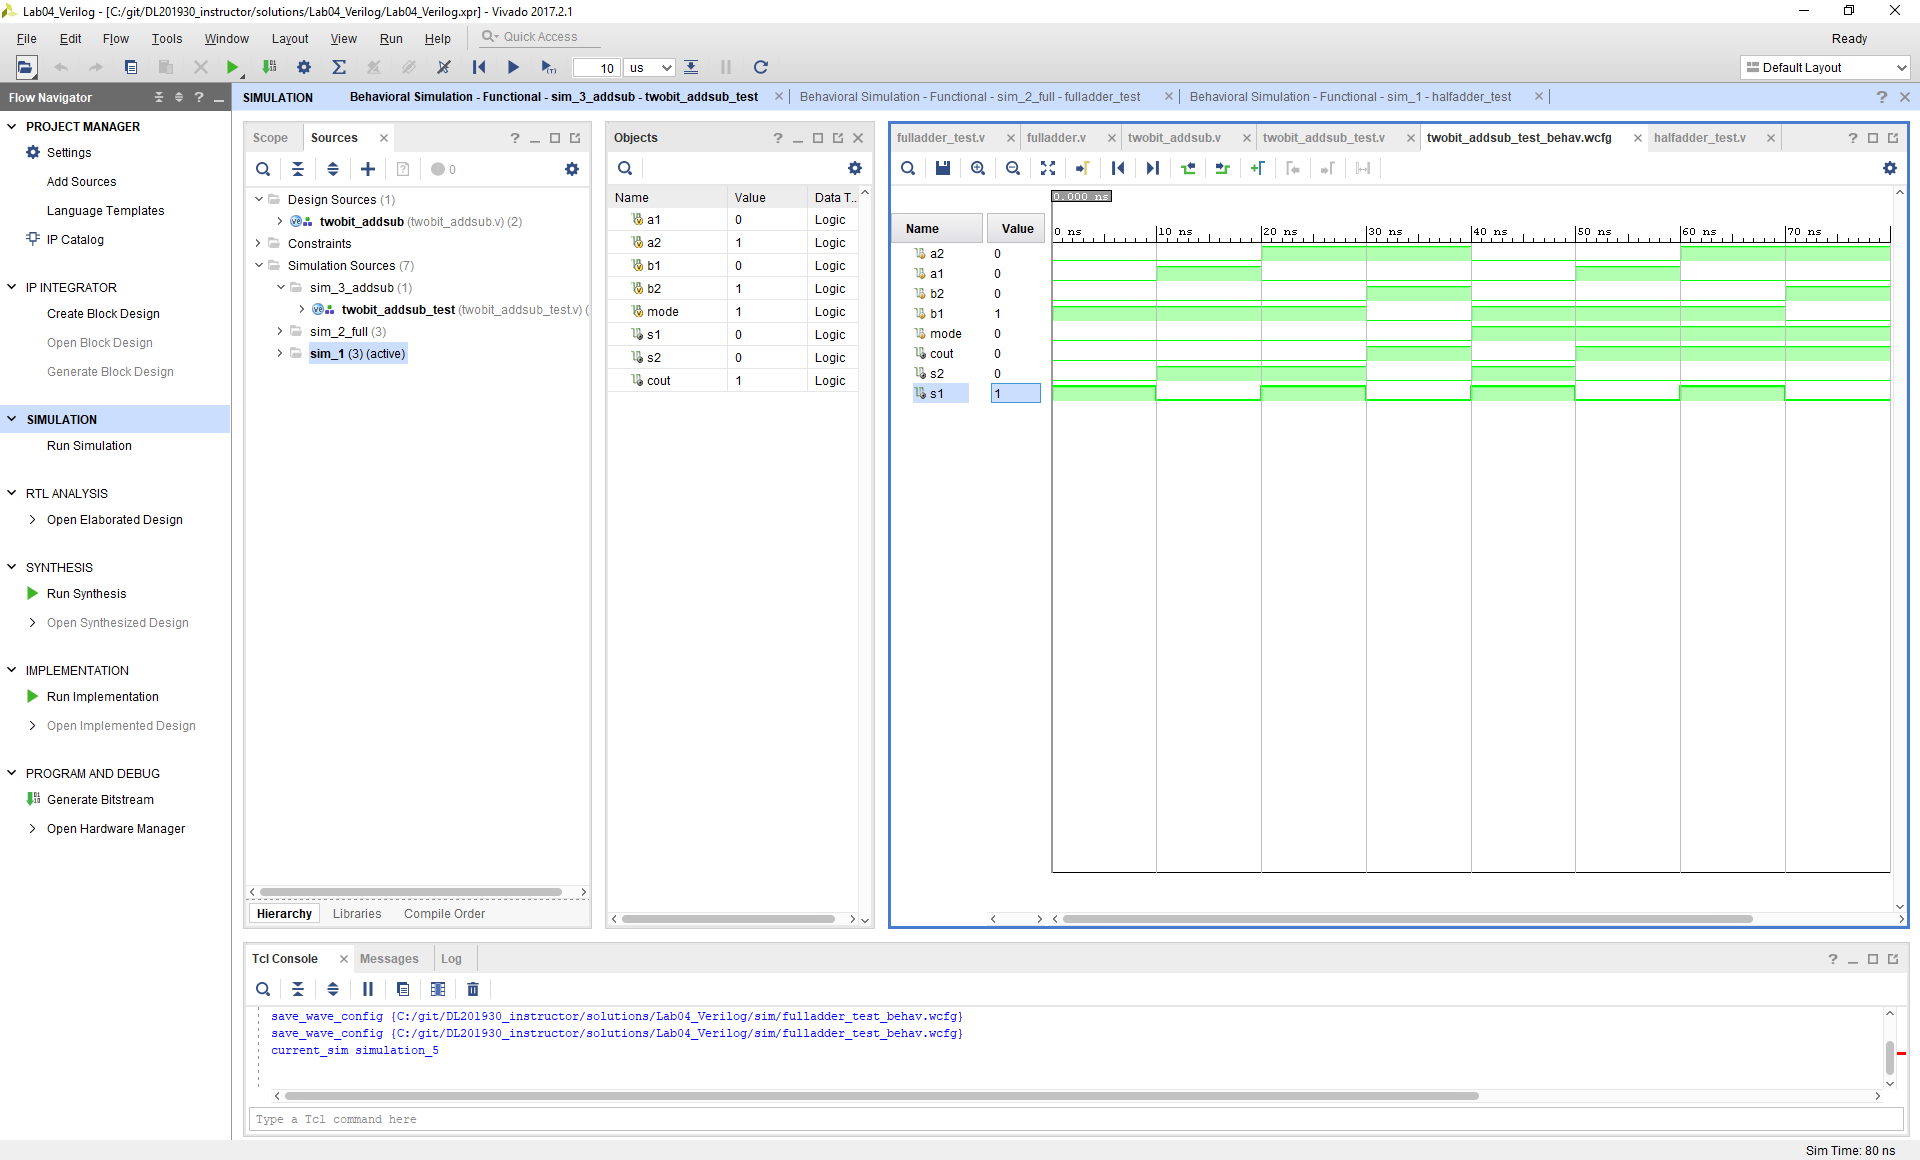
\includegraphics[width=1.0\textwidth, trim=19cm 15cm .5cm 4cm,clip]{lab1_example_screenshot.PNG}
\end{center}	
\begin{center}
Figure 1.1: Table and simulation waveform to reproduce 
\end{center}
	
	
\section*{Code}
module example
\#(parameter BITS=4)
(
input [BITS-1:0] in0, in1,
input sel,
output [BITS-1:0] out
);

// Choose in1 or in0
out = sel ? in1: in0; 
endmodule
\end{document}
